\section{Theorie}
\label{sec:Theorie}

\subsection{Die Grundlagen aus der Quantenmechanik und Optik}
\label{sec:t1}
Um die Versuche um die Quantenschlüsselung zu verstehen, ist eine gewisse Basis 
aus der Quantenmechanik und Optik unumgänglich. So folgt aus dem Welle-Teilchen-
Dualismus, dass Licht sowohl Wellen- als auch Teilcheneigenschaften besitzt. 
Ebenso existiert die Unschärferelation, welche es unmöglich macht, die genaue 
Position und den Impuls eines Teilchens gleichzeitig zu bestimmen. Wenn ein Photon 
gemessen wird, kollabiert seine Wellenfunktion, was bedeutet, dass es sich in einem
bestimmten Zustand befindet (Kopenhager Deutung). 
\vspace{0.5cm}
\\
\noindent Die Polarisation von Photonen spielt eine zentrale Rolle für das Experiment.
Darunter versteht sich die Schwinungsrichtung der elektromagnetischen Welle, wie 
es Licht ist. Grundsätzlich gibt es verschiedene Arten von Polarisation, wie
lineare, zirkulare und elliptische Polarisation. Unpolarisiertes Licht besteht aus
Photonen, die in alle möglichen Polarisationen schwingen, während polarisiertes 
Licht Photonen enthält, die in einer bestimmten Richtung schwingen. Für dieses 
Experiment ist die lineare Polarisation relevant, da sie zur Kodierung von 
Informationen verwendet wird. Darunter ist die Schwingungsrichtung der elektromagnetischen
Welle zu verstehen, welcher in einer Ebene liegt. Eine Veranschaulichung befindet 
sich in \autoref{fig:t1}
\begin{figure}[H]
    \centering
        \centering
        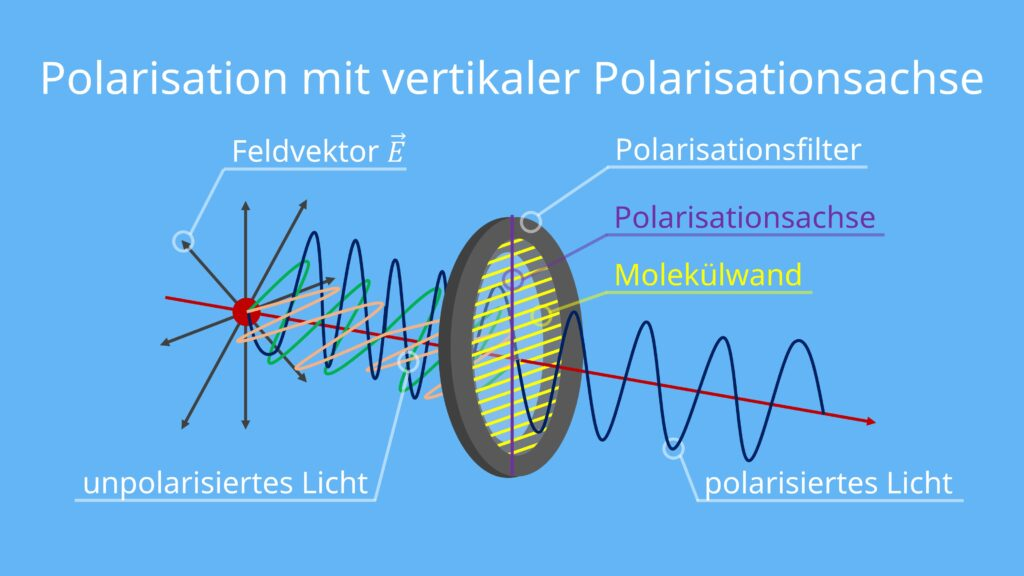
\includegraphics[width=0.75\textwidth]{Bilder/Polarisation.jpg}
        \caption{Lineare Polarisation an einem Filter. \cite{Polarisation}}
    \hfill
    \label{fig:t1}
\end{figure}


\subsection{Das BB84-Protokoll}
Das BB84-Protokoll ist ein Verfahren, welches die sichere Übertragung von
Informationen ermöglicht, indem es die Prinzipien der Quantenmechanik nutzt. Es gibt 
das Modul des Senders (Alice genannt) und des Empfängers (Bob genannt), sowie die 
Möglichkeit eines Abhörers (Eve). Von Alice werden Photonen gesendet und auf einen 
Strahlteiler geleitet, welcher die Photonen auf zwei verschiedene Detektoren leitet.
Hier werden entweder das Bit 0 oder 1 empfangen, abhängig von der Polarisation der
Photonen. Umittelbar hinter dem Laser von Alice befindet sich ein Polarisationsfilter,
welcher die Bits in 2 Basen mit jeweils 2 Zuständen kodiert. Eine Übersicht ist in 
\autoref{fig:t2} zu sehen.
\begin{figure}[H]
    \centering
        \centering
        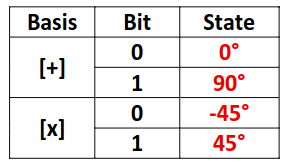
\includegraphics[width=0.4\textwidth]{Bilder/ecs.png}
        \caption{Encoding Tabelle für das BB84-Protokoll. \cite{anleitung14}}
    \hfill
    \label{fig:t2}
\end{figure}
\noindent Das Modul von Bob verfügt ebenfalls über Polarisationsfilter sowie 
Strahlteiler und Detektoren, um die Photonen zu messen. 
\\
Um Nachrichten sicher zu übertragen, wird mittels One-time-pad eine Verschlüsselung
vorgenommen. Dazu werden von Alice willkürliche Signale gesendet, sowohl der Bit 
als auch die Basis werden zufällig gewählt. Bob empfängt die Signale ebenfalls in
einer zufälligen Basis. Nach der Datenübermittlung wird die Sifting Phase eingeleitet,
in der überprüft wird, welche Basen von Bob und Alice übereinstimmen. In allen anderen 
Fällen werden die Daten verworfen. Die verbleibenden Daten bilden den Raw Key, mit 
dessen Hilfe nun die eigentlichen Nachrichten verschlüsselt versendet werden können.
\\
Ein Beispiel:
\begin{table}[H]
    \centering
    \caption{Experimentell ermittelte Ergebnisse.}
    \label{tab:t1}
    \begin{tblr}{
        colspec = {c c c c c},
        row{1} = {guard, mode=math},
    }
    \toprule
    \text{Messung} & \text{Alice Basis} & \text{Bob Basis} & \text{Alice Bit} & \text{Bob Bit} \\
    \midrule
    1 & + & + & 0 & 0 \\
    2 & x & + & - & - \\
    3 & + & x & - & - \\
    4 & + & + & 1 & 1 \\  
    \bottomrule
    \end{tblr}
\end{table}
\noindent Haben Alice und Bob die gleiche Basis gewählt, so stimmen die Bits überein
und können für die Verschlüsselung verwendet werden. Das funktioniert, da Bobs 
Strahlteiler die Photonen entsprechend der Polarisation auf die Detektoren leitet. 
Stimmt die Basis also überein, dann werden auch die gleichen Bits detektiert. 
Sobald der Raw Key generiert ist, können die Nachrichten gesendet werden. Es gilt 
\begin{align}
    \text{Nachricht} \oplus \text{Raw Key} &= \text{Verschlüsselte Nachricht} \\
    \text{Verschlüsselte Nachricht} \oplus \text{Raw Key} &= \text{Nachricht}.
\end{align}
Soll etwa der Buchstabe A \cite{Ainbinär} verschlüsselt werden, so ergäbe sich:
\begin{align*}
    \text{A}: 01000001 \\
    \text{Beispielhafter Raw Key}: 10100101 \\
    \text{Verschlüsselte Nachricht}: 11100100
\end{align*}
\vspace{0.5cm}
\\
\noindent Neben Alice und Bob kann ein Modul für einen Abhörer (Eve) in den 
Strahlengang eingebaut werden. Um diesen zu detektieren, wird die Fehlerrate der 
übereinstimmenden Basen bestimmt. Ohne einen Abhörer liegt die Fehlerrate bei 0\%,
da alle Bits bei übereinstimmender Basis korrekt übertragen werden. Sobald Eve
eingebaut wird, wird hier jeder Puls in einer zufälligen Basis gemessen. Wenn die 
Basis identisch zu der von Alice gewählten Basis ist, dann wird der Puls korrekt
gemessen und weitergeleitet. Ist die Basis unterschiedlich (Was in 50\% der Fälle
vorkommt), wird ein zufälliges Bit gemessen und an Bob weitergeleitet, welcher 
wiederum in einer zufälligen Basis misst. Die Kombination dieser zufälligen 
Ereignisse führt dazu, dass nach dem Basisabgleich etwa 25\% der Bits zwischen 
Alice und Bob nicht übereinstimmen. Ein Anstieg der Fehlerrate auf diesen Wert ist
daher ein Indiz für einen Abhörversuch. In der Praxis wird dafür ein Teil der 
Messwerte geopfert, um die Fehlerrate zu bestimmen. Berechnet wird die Fehlerquote 
mittels
\begin{equation}
    \text{QBER} = \frac{N_\text{error}}{N_\text{sifted bits}}.
\end{equation}

\subsection{PNS Attacke und decoy states}
Eine in der Theorie relevante Angriffsform ist die Photon Number Splitting (PNS)
Attacke. Dabei nutzt Eve aus, dass reale Laserquellen manchmal Pulse mit mehreren
Photonen aussenden. Sie führt eine Quanten-Non-Demolition-Messung durch, um die
Photonenzahl zu bestimmen: Bei Ein-Photon-Pulsen blockiert sie das Signal, bei
Mehr-Photon-Pulsen behält sie ein Photon für sich und lässt den Rest passieren.
So können am Modul von Eve Informationen gewonnen werden, ohne dass Alice und Bob
dies bemerken.
\vspace{0.5cm}
\\
\noindent Um sich gegen diese Angriffsform zu schützen, können sogenannte decoy
states verwendet werden. Die Grundidee besteht darin, dass Alice nicht nur einen
einzigen Pulstyp verwendet, sondern drei verschiedene Typen mit unterschiedlichen 
mittleren Photonenzahlen, die für Eve nicht unterscheidbar sind: den signal state
mit der Intensität $\mu$ (dieser wird später für die Schlüsselgenerierung verwendet), 
einen oder mehrere decoy states mit einer niedrigeren Intensität $\nu$ sowie den
vacuum state mit der Intensität 0 (dieser dient zur Bestimmung des Untergrundrauschens).
Alle Zustände werden von Alice zufällig ausgewählt und auf die gleiche Weise kodiert.
Für Eve ist es unmöglich zu erkennen, ob ein Puls ein Signal oder ein decoy ist.
Bei jedem Datensatz werden zwei elementare Größen bestimmt: die QBER und der Gain.
Der Gain $Q_i$ ist die Wahrscheinlichkeit, dass Bob einen Puls detektiert, wenn von
Alice ein Puls vom Typ $i$ gesendet hat. Durch den Vergleich der Gains und QBERs von
signal- und decoy-Pulsen können Alice und Bob die Beiträge von Ein-Photon-Pulsen von
denen der Mehr-Photon-Pulse trennen. Gelingt dies, lässt sich ein sicherer Schlüssel
allein aus den Ein-Photon-Ereignissen gewinnen, selbst wenn Eve alle Mehr-Photon-Pulse
kennt.
\\
Im hier verwendeten Thorlabs-Experiment wird die decoy state Methode nicht in dieser
vollständigen Form realisiert, sondern mit zwei verschiedenen Wellenlängen (roter 
und grüner Laser). Bestimmte Kombinationen aus Wellenlänge, Basis und Polarisation 
werden als decoy states definiert, siehe dazu \autoref{fig:t3}. Alice sendet speziell 
kein grünes Licht bei einer Polarisation von 90° und ebenso kein rotes Licht bei 
einem Zustand von 45°. Erscheinen sie dennoch bei Bob in der Detektion, deutet das 
auf eine Störung des Kanals hin: den experimentellen Fehler, verursacht durch Eves 
Messung.
\begin{figure}[H]
    \centering
        \centering
        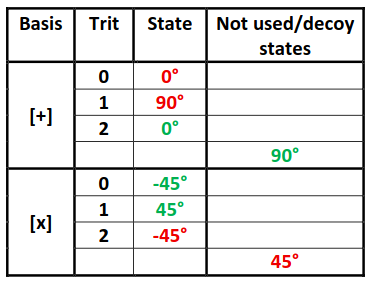
\includegraphics[width=0.6\textwidth]{Bilder/ternär.png}
        \caption{Encoding Tabelle für das ternäre BB84-Protokoll bei zwei Wellenlängen.
        Es existieren nur r0+, r1+, g2+, r0x, r1x und r2x Zustände. \cite{anleitung14}}
    \hfill
    \label{fig:t3}
\end{figure}


\subsection{Fehlerrechnung}
Die gemessenen Werte unterliegen Messunsicherheiten und werden demnach im
Folgenden nicht als fehlerfrei angesehen. Die Fehler entstehen bei der
Bildung der Mittelwerte durch den Fehler des Mittelwerts und bei der
Regressionsrechnung sowie der Fehlerforpflanzung durch Python.
Der Mittelwert ist definiert durch
\begin{equation}
    \overline{x} = \frac{1}{N} \sum\limits_{i=1}^N x_i.
\end{equation}
\noindent Der statistische Fehler des Mittelwerts ist somit gegeben durch 
\begin{equation}
    \begin{aligned}
        \increment \overline{x} &= \sqrt{\overline{x^2\kern-0.1em} - \overline{x}^2} \\
                            &= \frac{\sqrt{\frac{1}{N-1} \sum\limits_{i=1}^N (x_i - \overline{x})^2}}{\sqrt{N}}.
    \end{aligned}
\end{equation}
Um Fehler einzubeziehen, wird die Gauß'sche Fehlerfortpflanzung verwendet:
\begin{equation}
    \label{eqn:9}
    \increment f = \sqrt{\left(\frac{\partial f}{\partial x}\right)^2 \cdot \left(\increment x\right)^2 + \left(\frac{\partial f}{\partial y}\right)^2 \cdot \left(\increment y\right)^2 + .... + \left(\frac{\partial f}{\partial z}\right)^2 \cdot \left(\increment z\right)^2}
\end{equation}